
\documentclass[runningheads]{llncs}
\usepackage{tikz}
\usetikzlibrary{bayesnet}
\usepackage{amsmath}
\usepackage{amsfonts}
\usepackage{rotating}
\usepackage{graphicx}
\usepackage{subfigure}
\usepackage{tikz}
\usepackage{multirow}
\usepackage[linesnumbered,boxed]{algorithm2e}
\usepackage{cite}
\setlength{\abovecaptionskip}{10pt}
\setlength{\belowcaptionskip}{-10pt}
\newcommand{\Ep}{\mathbb{E}}
\newcommand{\Real}{\mathcal{R}}
\newcommand{\Gaussian}{\mathcal{N}}
\usepackage{graphicx}


\begin{document}
%title change
\title{Model Sentiment Evolution For Social Incedents}
\author{Yunjie Wang\inst{1} \and Chen Lin\inst{1}}

\authorrunning{Y.Wang et al.}

\institute{Department of Computer Science, Xiamen University, China \email{chenlin@xmu.edu.cn}}

\maketitle             

\begin{abstract}
Tracking opinion over time is a powerful tool that can be used to detect the possible reasons of a sentiment change. In this paper, we focus on the problem of tracking sentiment changes caused by social events and find the time point where the sentiment is mutated. For a social event, the traditional sentiment outlier detection method focuses on transforming the sentiment polarity of all tweets related to the event into sentiment value of the event itself. For example,we can use the ratio of tweets with positive sentiments or the average of tweet sentiment values. Then detect the sentiment outliers by different ways, such as calculating residuals. We try to model public opinion evolution in a holistic framework and use probability to indicate the likelihood of sentiment mutation at each time point. Experimental results on  Weibo data set validate the effectiveness of the proposed model.


\keywords{Sentiment change  \and Outlier detection }
\end{abstract}
%
%
%
\section{Introduction}
%Motivation
Nowadays Microblogging has become the major platform for Chinese people to publish information and share opinions about social incidents. Public opinion on Microblogging platforms has greatly influenced the Chinese society, sometimes even change the investigation and judicial outcome~\cite{{Cheung2014Battle}}. 
For example, in the ``Jiang Ge'' incident, a Chinese female student was killed in Japan, and her friend witnessed all this without providing any help. This event caused great anger on the Microblogging, which made the criminals got the punishment he deserved. %change 
The power of public opinion in Microblogging space make it appealing to analyze sentiment evolution for social incidents in microblogs for individuals, enterprises, NGO organizations , researchers, and government officials and so on.

%Problem studied
In this paper, to facilitate understanding of public opinions, we focus on the problem of modeling sentiment evolution for social incidents. 
Given a sequence microblogging comments related to any social incident, our goal is to reveal the sentiment evolution pattern related to the involved entities in this incident and identify the significant sentiment shifts. 
As shown in Fig.~\ref{fig:tweet}, for comments on the "Jiang Ge" incident, we analyze the public opinion and visualize. %more specific, better describe the incident first

%first layer: input sequence from left to right, balanced text size
%input: background tweets in each time slice 1~2
%second layer output entity-specific sentiment polarity +- bar graph , aim to visualize evolution
%third layer  entity specific vocabulary
%forth layer shift, background tweet 

\begin{figure}
    \centering
    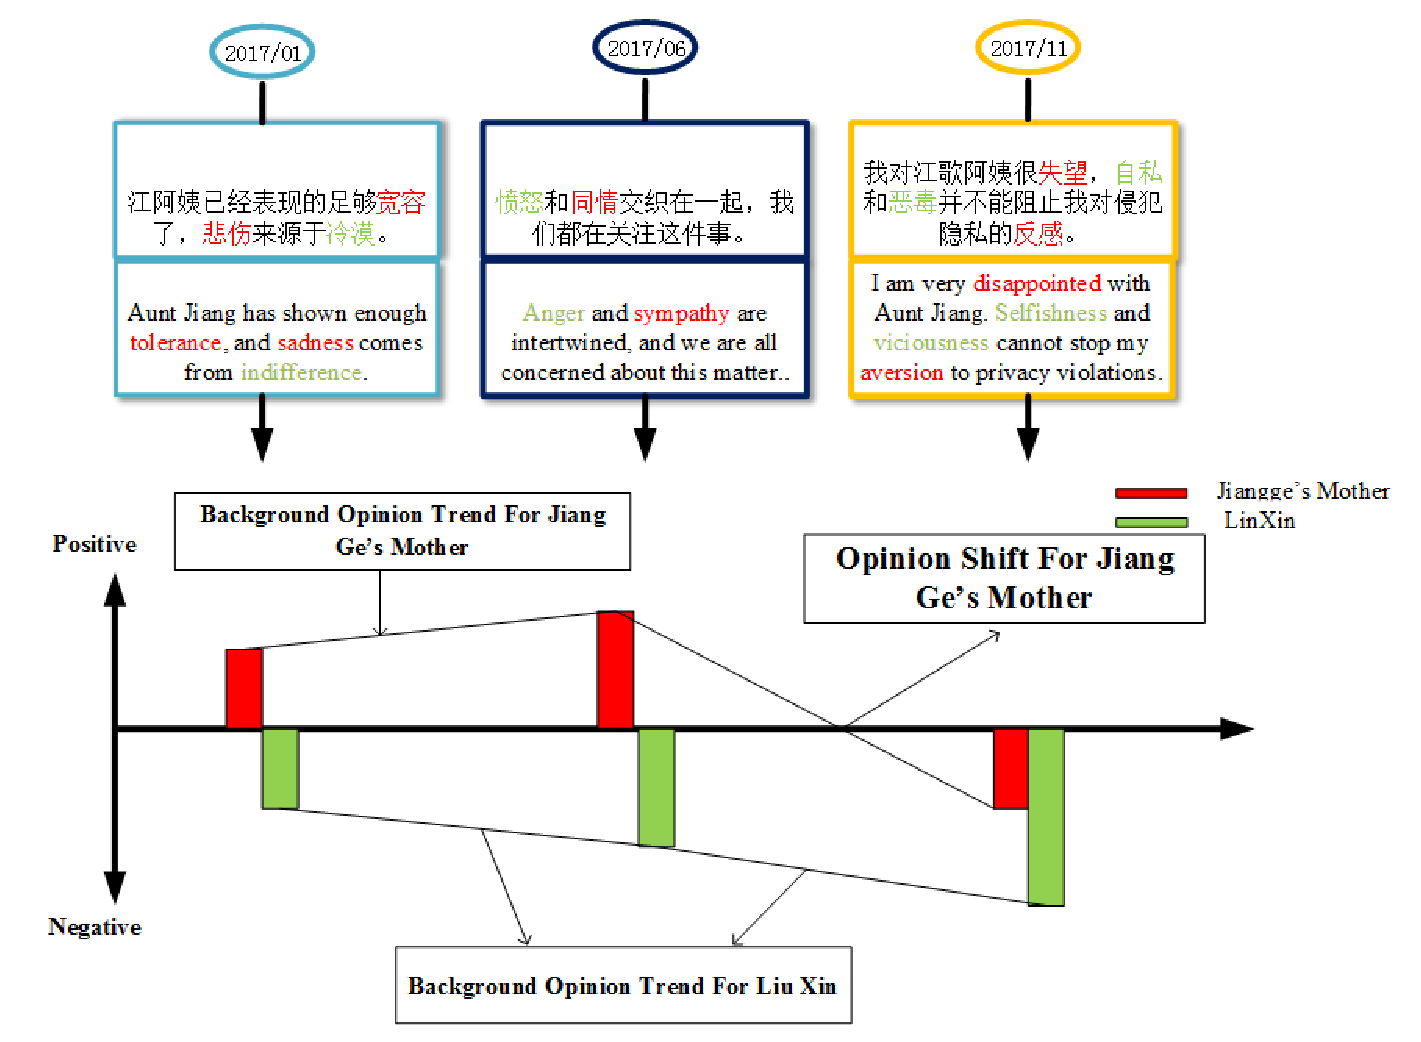
\includegraphics[width=1.0\textwidth,height=3.5in]{tweet.eps}
    \setlength{\abovecaptionskip}{-0.1cm}
    \caption{Comments from ``Jiang Ge'' incident and reflected characteristics of social incident}\label{fig:tweet}
\end{figure}

%Related work
Recently there is an increasing interest in tracking microblogging sentiments for entities~\cite{Giachanou2016sentichange,Giachanou2017sentichange} or topics~\cite{Tsytsarau2014Topics,Thelwall2011topic}. Most of them are based on a two stage framework, i.e. first adopt a sentiment extraction tool such as SentiStrength~\cite{sentistrength2010} to compute the sentiment score for an entity or topic, then conduct statistical analysis such as outlier detection to obtain sentiment spikes. However, modeling public opinion for social incidents poses several challenges that haven't been addressed by previous research.

%mixed feelings
The first challenge is to \textbf{identify entity-level sentiment}. 
As a social incident often involves several entities (i.e. people or organizations), extracting entity level sentiment is important.
For example, as shown in Fig~\ref{fig:tweet}, in ``Jiang Ge'' incident, people has negative sentiment to the Liu Xin, a person who witnessed her friend being killed and indifferent, positive sentiment to the Jiang Ge's mom. % redundant
Existing research utilizes coarse-grained analysis to obtain an averaged sentiment for an event without separating different entities, which is clearly problematic.%second layer
This is not a trivial problem because the length limit of microblogs encourage people to use short and informal expressions.
As in Fig.~\ref{fig:tweet}, multiple opinion expressions are put in a sentence which targets towards different entities. %running example, figure circle, as shown in ?? 
To address this challenge, it is helpful to embed proximity information to enhance entity-level sentiment extraction accuracy. 

%noisy lexicon
The second challenge is to \textbf{filter an accurate lexicon}. 
In the literature there are two types of sentiment extraction methods: supervised and lexicon based.
Due to the dynamic nature of social incidents (i.e. happen suddenly, constantly changing), it is infeasible to label real-time training corpus. %
Lexicon based sentiment extraction is widely adopted~\cite{sentistrength2010,Thelwall2012lexicon,Ortega2013lexicon}. 
A lexicon is a collection of words with negative and positive sentiments to compute the final polarity of sentiments. 
Lexicon based methods do not require a training dataset and are easy to implement. 
However, the problem is that using one lexicon for all incidents is too general and noisy. %noisy
For example, in Figure~\ref{fig:tweet}, a general lexicon consists of 13 sentiment words (in blue), while four of them (in red) are irrelevant to this incident. Including them in the lexicon will harm the performance of sentiment extraction.
Hence it is necessary to construct a minimal ``global'' vocabulary with high precision and an incident specific lexicon without supervision.

%background evolution + shift
The third challenge is to \textbf{simutanously model the evolution of sentiment background and sentiment shift}.
In previous work, researchers mostly depend on statistical analysis such as outlier detection to detect sentiment spikes~\cite{Giachanou2016sentichange,Giachanou2017sentichange,Giachanou2016sentitime}.
Such an method is not sufficient, because the evolution of the background is largely overlooked.
The fact that events are continuously changing causes changing responses in public opinions. Hence sentiment shift should be distinguished with the evolution patterns of background sentiment.  
For example, in Figure~\ref{fig:tweet}, the background sentiment towards Jiangge's mom is an increasing trend of positive sentiment. Revealing this evolution pattern marks the significance of sentiment shift at the third time point. %running example
In this article we propose a probabilistic model that simultaneously model the evolution of background opinion and the opinion shifts.

%contributions
Our contributions are three folds. 
We investigate the impact of proximity information in obtaining entity-level sentiment extraction.
We design an efficient algorithm to extract global lexicon and incident specific lexicon.
In the model aspect, we propose to simutanously model the evolution of opinion and opinion shift.

This paper is organized as follows. We briefly survey the related work in Sec.~\ref{sec:related}. In Sec.~\ref{sec:problem definition} to Sec.~\ref{sec:public opinion model}, we describe the methodology. We present and analyze the experimental results on a real data set in Sec.~\ref{sec:Experiment}. We conclude our work and suggest future directions in Sec.~\ref{sec:conclusion}.
\section{Related Work}\label{sec:related}
%sentiment tracking
\textbf{Sentiment Tracking on Microblogs} has received considerable attention from both academy and industry~\cite{Giachanou2016sentichange,Giachanou2017sentichange,Giachanou2016sentitime,An2014sentimentchange,Bollen2011sentimentchange,Tan2014topic,Montero2016sentimentchange}. Most of existing work adopt a cascade framework, i.e. in the first step sentiment of each tweet is extracted, in the second step sentiment shift is detected~\cite{Giachanou2016sentichange,Giachanou2017sentichange,Giachanou2016sentitime,An2014sentimentchange,Bollen2011sentimentchange,Tan2014topic}. To extract sentiment, the collection of tweets are divided into numerous time slices, and the ratio of positive and negatie sentiments is computed in a time slice~\cite{Giachanou2017sentichange,Giachanou2016sentitime,An2014sentimentchange,Bollen2011sentimentchange}. 
To detect sentiment shift, residual between actural and predicted sentiment value is the most commonly adopted measurment~\cite{Giachanou2016sentichange,Giachanou2016sentitime}. 
Furthermore, topic information is incorporated in recent studies. Sentiment change is represented by topic changes in~\cite{Tan2014topic}, an integrate framework based on empirical heuristics is utilized in~\cite{Montero2016sentimentchange} to identify
the emotional spikes and locate causes of spikes.%integration 

%sentiment analysis
A fundamental block in sentiment tracking systems is \textbf{sentiment analysis}. In the literature, there are two types of sentiment analysis algorithms: supervised learning and lexicon-based methods~\cite{Ahmed2017SentiCR}. \textbf{Supervised learning method} creates a training model based on training data
to classify the sentiment polarity of sentences. Obtaining training data and selecting features are the two most important parts of this methods. 
Emoji is often used to label sentiments of tweets~\cite{Go2009Supervisedlearning,Pak2010Supervisedlearning}. Hashtag is another major source to label training data~\cite{Papadopoulos2012SocialEvent}.
But the accuracy of label by emoji is low. To overcome this issue, an ensemble of sentiment detection tools is employed to obtain the training data~\cite{Barbosa2010Supervisedlearning}. 
The goal of supervision based methods is to classify the polarity of sentiments. To obtain a high precision, lexical features such asu nigrams and POS~\cite{Go2009Supervisedlearning,Davidov2010Supervisedlearning}, syntax features  such as  retweets, URLs, emoticons, and meta-features such as  POS tags, words’ polarity,~\cite{Barbosa2010Supervisedlearning} are obtained.
Experiments have shown that classifiers benefit most from features which involve text polarity~\cite{Agarwal2010Supervisedlearning}.

Due to the lack of training data, most researchers turn to \textbf{lexicon based methods}. 
SentiStrength is the first open domain large-scale lexicon, which is used as a baseline in most sentiment detection algorithms like SentiStrength2~\cite{Thelwall2012lexicon}, SentiStrength-SE~\cite{Rakibul2017SentiStrength-SE}, and VADER~\cite{Hutto2014SSimproved}. 
SentiSterength2~\cite{Thelwall2012lexicon} improves the accuracy of SentiStrength by adding idioms. 
VADER~\cite{Hutto2014SSimproved} improves the accuracy of SentiStrength by grouping sentiment words on Twitter and manually filtering them. 
SenciStrength-SE improves the recall of SentiStrength by designing different lexicons for different domains~\cite{Rakibul2017SentiStrength-SE}. 
The above methods are based on static lexicons.
Recently,we've seen an emerging attempt to construct dynamic lexicon. 
For example, to enclose subtle dimensions of a word’s sentiment, a seed lexicon is defined in ~\cite{Feng2011lexicon} and connotation lexicon is retrieved based on PageRank and HITS. 
However, such a connotation lexicon is still noisy and often not scalable, because it contains sentiment words that are not related to any entity in an event.


%architecture
\section{Problem Definition}\label{sec:problem definition}
Social events are planned by people, attended by people and that the media illustrating the events are captured by people~\cite{Papadopoulos2012SocialEvent}. So social events involve interactions between different entities. Social events are dynamic and occur in a limited time. Emotional changes contained in social events tend to be regular. These features result in sentiment analysis and sentiment tracking methods previously used on entities and topics that no longer apply to social events. We use a new opinion model to simulate the evolution of public opinion in social events and to find the time points when sentiments shift suddenly during the evolution. In order to achieve the best results of our model, we consider the impact of the entity on the results of sentiment analysis, and use the core lexicon and feature lexicon to construct a unique lexicon of each event to improve the accuracy of sentiment classification.



\section{Entity-level Sentiment Classification}\label{sec:sentiment classification}
%framework
Our goal here % two-steps
is to extract a global lexicon for all incidents, incident specific lexicon. %lexicon
incorporate distance information in sentiment classification. 

We have improved two aspects to increase the accuracy of sentiment classification:  (1)We use the core lexicon and feature lexicon to construct a unique lexicon of each event. (2) We add entities to the process of sentiment classification.
\subsection{Core Lexicon And Feature Lexicon}
Given a set of candidate sentiment words $W$ with labeled sentiment polarity $P$, we aim to select a minimal global lexicon for all events.  

\textbf{Graph construction}:  $G=\{V,E\}$, where each node $v\in V$ represents a word $w\i W$ in the corpus and remove the neutral words, low frequency words and stop words to get the candidate lexicon.  If two words appear in the same sentence, then there is an edge between the nodes corresponding to the two words. Traversing the corpus of several events, getting the graph corresponding to these events. 

\textbf{Global lexicon $U$ extraction}: inspired by ~\cite{Zhang2012corenodes}, a node $u$ is added to the global lexicon $U$ if $d(u)\geq \max\{d(v)|v\in N(u)\}$,  node having a greater degree than all of its adjacent nodes. 

\textbf{Incident specific lexicon $Q$}: compute pair-wise similarity $s(i,j), i,j\in V$. $U$ $l(i,j)=\max {s}$ top . 

\begin{equation}
    s(i,j) = \frac{2*|Edeg(adj(i)\cap adj(j))|}{|(adj(i)\cap adj(j)|*(|(adj(i)\cap adj(j)|-1)}
\end{equation}
$adj(A)$ is the set of nodes adjacent to A, adj(A) $\cap$ adj(B) is the common nodes of adjacent nodes of A and adjacent nodes of B. Edge(adj(A) $\cap$ adj(B)) stands for the edges linked by the nodes in adj(A) $\cap$ adj(B).%modification on notations


\subsection{Distance Function}
Here, we describe how to add entities to the process of sentiment classification. We use entities as the granularity of sentiment classification. We believe that in one sentence, the sentiment words in different positions have different effects on the entity. Sentiment words that are close to the entity have a greater influence on the sentiment polarity of the sentence than the sentiment words far from the entity. We use the average of all sentiment words on the entity as the sentiment polarity of the sentence.

We use the distance function to calculate influence of sentiment words on entities. Following some previous work, We use four kernel functions as the form of the distance function in turn: Gaussian, Triangle, Cosine, and Circle:

\textbf{1. Gaussian kernel}
\begin{equation}
    k(i,j) = \exp\left[\frac{-(i-j)^2}{2\sigma^2}\right]
\end{equation}

\textbf{2. Triangle kernel}
\begin{equation}
k(i,j)=\begin{cases}
1-\frac{|i-j|}{\sigma} &\mbox{if $|i-j|\leq \sigma$}\\
0 &\mbox{otherwise}
\end{cases}
\end{equation}

\textbf{3. Cosine (Hamming) kernel}
\begin{equation}
k(i,j)=\begin{cases}
\frac{1}{2}\left[1+cos\left(\frac{|i-j|\cdot\pi}{\sigma}\right)\right] &\mbox{if $|i-j|\leq \sigma$}\\
0 &\mbox{otherwise}
\end{cases}
\end{equation}

\textbf{4. Circle kernel}
\begin{equation}
k(i,j)=\begin{cases}
\sqrt{1-\left(\frac{|i-j|^2}{\sigma}\right)} &\mbox{if $|i-j|\leq \sigma$}\\
0 &\mbox{otherwise}
\end{cases}
\end{equation}

$i$ is the position of the sentiment word in the sentence, and $j$ is the position of the entity in the sentence. All four of these kernel functions have only one parameter. We will determine the best form of the distance function and best value of the parameter in the experiment.

\subsection{Calculate Entity level Sentiment polarity}
Based on the above work, here we give the formula for calculating the sentiment value of a sentence. We first calculate the influence of one of the sentiment words on the entity.
\begin{equation}
    s_i = (-1)^n\cdot d_i\cdot v_i\cdot k(p_i,j)
\end{equation}
$i$ is the number of this sentiment word. $n$ is the number of gainsay words between this emotional word and the sentiment word before it. $d_i$ is the sum of the weights of the degree words between this sentiment word and the sentiment word before it. $v_i$ is the emotional value of this emotional word. $k$ is the distance function. $p_i$ is the location of this emotional word. $j$ is the location of the entity.

We calculate the influence of all sentiment words on the entity according to this formula, and take the average value as the sentiment value of the sentence. If the sentiment value is greater than 0, we think that the sentence has a positive emotion. If the sentiment value is less than 0, we think that the entity has a negative emotion.

\section{Public Opinion Model}\label{sec:public opinion model}
Dramatic real-world events are known to have the power to impact on public opinions and to cause shift on public attitudes. For example, assassinations of Martin Luther King created a cultural shift in attitudes on race issues. Thus we are motivated to analyze news and user generated contents on social networking platforms, model the evolution and shifts of public opinions,  exact common patterns and explain anomalies.

We first explore our options on modeling the evolution of public opinions. Before we go into the details, we have to list a few assumptions here. (1) We only consider bi-polarized opinions, i.e. each unit piece of social comment is pre-processed by some opinion classifiers to be either positive or negative. The unit to be processed can be a phrase about an entity, a sentence, or a minimal length semantic unit. (2) We consider there is a background opinion distribution, i.e. how users normally react to a certain entity or a particular event. The background is smoothly and slowly changing, e.g. the public opinion for civil rights is constantly changing. (3) However, sometimes a new piece of evidence might trigger a sudden shift on public opinions, e.g. the assassination of Martin Luther King boosts public  supports to civil rights.  

\begin{figure}
  \centering
  \tikz[scale=0.5]{ %
%hypers
    \node[const] (a) {$a$} ; %
        \node[const,right = of a] (b) {$b$} ; 
        \node[const,right = of b](sigma){$\sigma^2$};
        
%emotion evolutions        
  \node[latent, below = of b](gamma){$\gamma$};

   \node[latent, below = of sigma](alpha0){$\alpha_0$};
     \node[const, right = of alpha0](alphadots){$\cdots$};
   \node[latent, right = of alphadots](alphat){$\alpha_t$};
    \node[latent, right = of alphat](alphatp){$\alpha_{t+1}$};
    
    \edge{a}{gamma};
     \edge{b}{gamma};
     
      \edge{sigma}{alpha0};
    	\edge{sigma}{alphat};
	\edge{sigma}{alphatp};
	\edge{alpha0}{alphadots};
	\edge{alphat}{alphatp};
    
  	\node[latent, below = 1 of gamma] (s0) {$s_{0,n}$};
%	 \node[latent, below = 0.8 of alpha0] (eta0) {$\eta_0$};
       	\edge{gamma}{s0};
%    	\edge{alpha0}{0};        
	

%	 \node[latent, below = 0.8 of alphat] (etat) {$\eta_t$};
	 		\node[latent, right = 2.8 of s0 ] (st) {$s_{t,n}$};
        	\edge{gamma}{st};
%            	\edge{alphat}{etat};

	
        \node[latent, below = 2 of alpha0 ] (y0) {$y_{0,n,m}$};
            \node[latent, below = 2  of alphat ] (yt) {$y_{t,n,m}$};
       	\edge{s0}{y0};
	\edge{alpha0}{y0};
	    	\edge{st}{yt};
	\edge{alphat}{yt};
	
	 \plate[inner sep=0.1cm, xshift=-0cm, yshift=0 cm] {O0} {(y0)} {$M_n$};
		 \plate[inner sep=0.1cm, xshift=-0cm, yshift=0.12 cm] {S0} {(s0)  (O0) } {$N_0$}; 

		 \plate[inner sep=0.1cm, xshift=-0cm, yshift=0 cm] {Ot} {(yt) } {$M_n$};
		 \plate[inner sep=0.1cm, xshift=-0cm, yshift=0.12 cm] {St} {(st)  (Ot) } {$N_t$}; 
	
        \node[latent, below = 2 of y0 ] (beta) {$\beta$};
        
       	\edge{beta}{y0};
	\edge{beta}{yt};
	   \node[latent, below = of beta](c){$c$};
	      \node[latent, right = of c](d){$d$};
   	\edge{c}{beta};
	\edge{d}{beta};
       
     }
 \caption{Plate notation of the proposed opinion evolution model}\label{fig:opinion}
\end{figure}
    
First we generate the prior distribution for the background opinion distributions. 
\begin{itemize}
\item For time $t=0$, sample  for the public opinion distribution, $\alpha_0\sim \Gaussian(0,\sigma^2 I)$.
\item For items $t=1: N$, sample $\alpha_{t+1}\sim \Gaussian(\alpha_t,\sigma^2)$. As $\Gaussian$ is a continuous and differentiable distribution, the evolution of background opinions is smooth and slow.
\item Generate a global prior for the switch, i.e. a variable that controls how likely the public opinion to change, by $\gamma\sim Beta(a,b)$
\end{itemize}


Note that all $\alpha$s  are vectors of real numbers, $\alpha\in \Real^2$. Next to generate the opinion distribution, we adopt $\pi(\cdot)$ function to convert $\alpha$ to a value within $(0,1)$, $\pi(\alpha_t)=\frac{\exp \alpha_{t,0}}{\exp \alpha_{t,0} + \exp \alpha_{t,1}}$.

For time $t$, with $N_t$ pieces of evidence, i.e. $N_t$ piece of news report published at time $t$, each evidence $n$ contains $M_n$ observations, e.g. user comments, we mimic the following generation process. 
\begin{itemize}
%\item Generate background opinion distribution $\eta_t \sim \pi(\alpha_t)$
\item For each pieces of evidence
\begin{itemize}
\item Generate a switch $s_t \sim Bern(\gamma)$
\item For each observation, generate $y_{t,n,m}\sim \begin{cases}
Bern(\pi(\alpha_t)) & \text{ if } s_{t,n}= 1\\ 
Bern(\beta) & \text{ if } s_{t,n}= 0 
\end{cases}$
\end{itemize}
\end{itemize}

The joint probability is given by
\begin{eqnarray*}
    p(\gamma,\beta,\alpha_0,\cdots,\alpha_T, \vec{s},\vec{y}, |a,b,c,d,\sigma^2) \\
    =    p(\gamma|a,b) p(\beta|c,d)  p(\alpha_{0:T}|\sigma^2) \prod_t \prod_ n p(s_{t,n}|\gamma) \prod_m p(y_{t,n,m}|s_{t,n},\alpha_t,\beta) 
    \end{eqnarray*}

However, as the above complete likelihood involves natural parameters $\pi(\alpha)$, we apply the lower-bound $\forall t, \ln (\exp \alpha_{t,0}+ \exp \alpha_{t,1}) \leq \ln \hat{\xi_t} + \frac{\exp \alpha_{t,0} + \exp \alpha_{t,1} -\hat{\xi_t}}{\hat{\xi_t}}$ to $p(y_{t,n,m}|s_{t,n},\alpha_t,\beta) = [\pi(\alpha_t)^{y_{t,n,m}} (1-\pi(\alpha_t))^{1-y_{t,n,m}}]^{s_{t,n}} [\beta^{y_{t,n,m}}(1-\beta)^{1-y_{t,n,m}}]^{1-s_{t,n}}$ whenever neccessary.
In the nutshell, the optimization algorithm is variational inference. Thus we make the following assumptions. 

\begin{equation*}
q(Z|\vec{y},a,b,c,d,\sigma^2) = q(\gamma|\hat{a},\hat{b}) q(\beta|\hat{c},\hat{d}) q(\alpha_{0:T}|\hat{\alpha_{0:T}})\prod_{t,n} q(s_{t,n}|\hat{e_{t,n}}) , 
\end{equation*}
where $Z$ includes all hidden variables, $\hat{e_{t,n}}\in \Real^2 $ is a vector. 

Then we implement the iterations over all hidden variables.

\section{Experiment}\label{sec:Experiment}
\subsection{Experimental Setup}
%crawl 
The data set used in our experiment is crawled through weibo API, collected between 2016 and 2018.through the microblogging API using keyword matching. %...crawl
The corpus includes 6 incidents, %top social incidents
 The tweets for each event are divided into news and corresponding comments. Details of the data set, including the description of each event, the number of news and comments are shown in Tab.~\ref{table:social event}.

In pre-processing, repeated tweets, emoji expressions, http links and mentions (@somebody) are removed from the data set.
Segmentation %

% \vspace{-0.6cm}
\begin{table}[ht]
\caption{Statistics of the data set}\label{table:social event}
\begin{center}
\tiny
\begin{tabular}{|l|l|l|l|}
\hline
Abbrevation   & Tweets & Time period (start end) & Event description                                           \\ \hline
JGmurder      & 368037 & 2016/11/02 2018/01/01   & Chinese female student Jiang Ge was killed in Japan         \\ \hline
CFfall        & 35081  & 2017/08/31 2017/10/16   & A maternal woman jumped died in the hospital                \\ \hline
RYBabused     & 35927  & 2017/11/23 2017/12/27   & Many children were abused in a kindergarten                 \\ \hline
HZbabysitter  & 167225 & 2017/06/22 2017/11/01   & A nanny in Hangzhou burned his employers                    \\ \hline
SDhumiliation & 17607  & 2017/03/25 2017/08/31   & A mother in Shandong was humiliated because she owed money. \\ \hline
WZXhospital   & 59501  & 2016/04/21 2016/09/11   & Wei Zexi died of fake medical information                   \\ \hline
\end{tabular}
\end{center}
\label{default}
\end{table}
% \vspace{-0.6cm}

\subsection{Sentiment Lexicon Extraction}
We first verify that the performance of lexicon construction.

%groundtruth
The ground truth is the polarity (positive v.s. negative) of sentiment words.
%pooling,3-5 comparative methods
 in manually generated. % 3 judges, label 
%majority vote


We choose precision, recall as evaluation metrics. The precision help us judge that how many words in the lexicon belong to sentiment words. The recall tell us the proportion of sentiment words in the lexicon to all sentiment words in the ground truth. We compare our method with PMI on sentiment lexicon extraction. PMI is a commonly used method that extends the seed lexicon by calculating pointwise mutual information of candidate words and sentiment seeds. The results are shown in Tab.~\ref{table:core lexicon}

% figure
% x: #tweets
% y: precision/recall/size
% comparative methods: 3-5 
%core + specific lexicon

% \vspace{-0.6cm}
\begin{table}[ht]
\caption{Comparative  of Core lexicon and PMI}\label{table:core lexicon}
\begin{center}
\begin{tabular}{|c|c|c|c|c|c|c|c|}
\hline
\multirow{2}{*}{Events} & \multirow{2}{*}{Tweet} & \multicolumn{3}{c|}{PMI}             & \multicolumn{3}{c|}{Core Lexicon}    \\ 
\cline{3-8}                         &                        & Precision & Recall & Size of Lexicon & Precision & Recall & Size of Lexicon \\ \hline
JGmurder                & 368037                 & 0.7179    & 0.7188 & 176             & 0.7936    & 0.7604 & 165             \\ \hline
HZbabysitter            & 167225                 & 0.7097    & 0.7750 & 101             & 0.7766    & 0.7833 & 94              \\ \hline
WZXhospital             & 59501                  & 0.6508    & 0.8289 & 60              & 0.8548    & 0.8158 & 62              \\ \hline
RYBabused               & 35927                  & 0.7083    & 0.7619 & 77              & 0.8077    & 0.8254 & 52              \\ \hline
CFfall                  & 35081                  & 0.4468    & 0.7015 & 75              & 0.8103    & 0.8557 & 58              \\ \hline
SDhumiliation           & 17607                  & 0.4074    & 0.7714 & 56              & 0.8484    & 0.9429 & 33              \\ \hline
\end{tabular}
\end{center}
\end{table}
% \vspace{-0.6cm}

Observing from Tab.~\ref{table:core lexicon}, we can see that our proposed approach is more effective for sentiment lexicon extraction than PMI. Among all six events, the core lexicon approach has higher precision than PMI, and among the five events, the core lexicon approach has a higher recall than PMI. More importantly, as the corpus of events becomes smaller, the precision of PMI shows a downward trend. PMI's precision on the two events with the smallest corpus is only 44 percent and 40 percent. At the same time, the PMI recall remained stable. This shows that as the event corpus becomes smaller, PMI sacrifices precision in order to extract emotional words as much as possible, resulting in a much larger lexicon than the lexicon obtained by the core lexicon method. Compared with PMI, as the corpus of events becomes smaller, the precision and recall of the lexicon obtained by the core lexicon method is increasing. Therefore, the lexicon extracted by the core lexicon method has better quality, especially when the corpus of events is small.

\subsection{Parameter Selection For Distance Function}
%groundtruth
Here we will get the form of the distance function and determine the parameters of the it through experiments. The experimental data set consisted of 2,000 tweets randomly selected from the corpus of six events. Manually mark the polarity of these tweets and determine the location of the entity by keyword. We use different distance functions to calculate the sentiment classification accuracy for the data set and systematically test a set of flxed $\sigma$ values from 1 to 30 in increments of 1. The results are shown in Fig.~\ref{fig:sigma}

\vspace{-0.5cm}
\begin{figure}
    \centering
    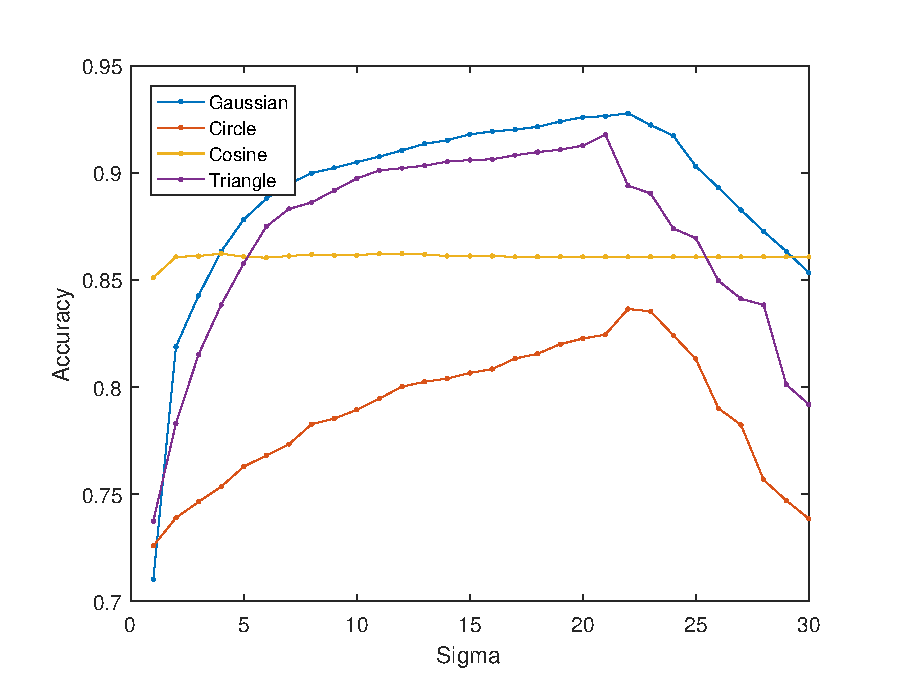
\includegraphics[width=0.5\textwidth,height=1.6in]{sigma.eps}
    \setlength{\abovecaptionskip}{-0.1cm}
    \caption{For different kernel functions, the relationship between sentiment analysis accuracy and $\sigma$}\label{fig:sigma}
\end{figure}

First, it is clear that adding entity to the process of sentiment recognition can improve the accuracy of sentiment classification. Among the four kernel functions, the Cosine kernel function is less affected by sigma. The accuracy of sentiment classification corresponding to the other three kernel functions increases first and then decreases, and all three kernel functions get the optimal value when sigma is equal to 21. The Gaussian kernel function performs best. So we take the Gaussian kernel function as a form of the distance function and set the value of sigma to 21. Under such conditions, the sentiment classification accuracy of the data set reached 92.77 percent.

\subsection{Evaluation of Sentiment Extraction}
Here, we show the impact of using the core lexicon and distance functions on sentiment classification. Before the experiment, we suspected that the distance function is more advantageous for long texts, because if a sentence contains few sentiment words, the distance of the sentiment words to the entity no longer has a strong influence on the classification results. In order to validate our conjecture, we randomly extracted three different lengths of comments from the event corpus to form three data sets. Manually annotate the emotional polarity of tweets in the dataset.

We compared our method to SentiStrength, SentiStrength-SE~\cite{Rakibul2017SentiStrength-SE} and SentCR. SentiStrength is a classic algorithm for sentiment classification. SentiStrength-SE has improved SentiStrength, this method designs different lexicon for events in different fields. SentCR is a supervised learning method designed for code review comments. We compared the sentiment classification accuracy of these four methods on positive and negative data set, and compared the impact of the length of the tweets on the classification results. The results are shown in Tab.~\ref{table:sentiment classification}

According to Table~\ref{table:sentiment classification}, Our approach has the best performance. On all dataset, our method's sentiment classification accuracy exceeds 80 percent, especially for negative dataset with tweets between 40 and 60 in length, the accuracy of our method is over 90 percent. There are many details in the table. We can see that except for SentCR, the accuracy of the other three methods on the positive dataset is lower than the accuracy on the negative dataset. This is because in our event, most of the comments contain a large number of negative words, but some of them are expressed in support of another person by expressing dislike of someone. Although there are many negative words in the tweet, the tweet still expresses positive emotions. Therefore, in our corpus, judging positive emotions is difficult to judge negative emotions. Despite this, our approach has achieved high accuracy on positive data sets. The accuracy of SentiCR remains stable because supervised learning methods are not affected by tweet semantics and structure. As the tweet grows longer, the accuracy of the our method using the distance function is significantly improved compared to the our method without using the distance function. So the distance function is more effective for long comments.

%figure
% \vspace{-0.6cm}
\begin{table}[ht]
\caption{Comparison of sentiment classification results}\label{table:sentiment classification}
\begin{center}
\begin{tabular}{|c|c|c|c|c|c|c|}
\hline
\multirow{3}{*}{Methods}             & \multicolumn{6}{c|}{Sentence length}                                                \\ \cline{2-7} 
                                     & \multicolumn{2}{c|}{0-20} & \multicolumn{2}{c|}{20-40} & \multicolumn{2}{c|}{40-60} \\ \cline{2-7} 
                                     & Positive    & Negative    & Positive     & Negative    & Positive     & Negative    \\ \hline
SentiStrength                        & 0.3774      & 0.5808      & 0.2254       & 0.3906      & 0.3938       & 0.3622      \\ \hline
SentiStrength-SE                     & 0.6014      & 0.6951      & 0.5040       & 0.5843      & 0.5752       & 0.6467      \\ \hline
SentiCR                              & 0.7953      & 0.7855      & 0.7911       & 0.7005      & 0.7404       & 0.7861      \\ \hline
xxx & 0.7279      & 0.7558      & 0.7517       & 0.7792      & 0.7477       & 0.7641      \\ \hline
xxx                           & 0.8477      & 0.8588      & 0.8539       & 0.8771      & 0.8862       & 0.9289      \\ \hline
\end{tabular}
\end{center}
\end{table}
% \vspace{-0.6cm}


\subsection{Evaluation of Public Opinion Model}
Here, we show the advantages of our public opinion model in simulating the evolution of public opinion. We set 19 time points for each event, with the same interval between each two time points. We use the core lexicon and feature lexicon to build a lexicon for each event, and calculate the sentiment polarity of each tweet in the corpus corresponding to each time point by the distance function.

%case study 


% \vspace{-0.6cm}

% precision
%comparative study
%overall 
We show the changes of the parameter $e$ in the Tab.~\ref{table:beta} The parameter $e$ represents the probability of a sudden change in public opinion at each time point. So we use the parameter $e$ to find the shift points in the sentiment change. For each event, we use the time point where the value of e is greater than 0.8 as the shift point. The ground truth of sentiment changes is obtained manually, we analyze the events at all time points and select the time points we believe can cause a sudden change in public opinion. We compare our model to the ground truth. The results are shown in Tab.~\ref{table:result}. Y represents this time point is considered to be a sentiment shift point. N is the opposite. As shown in Table~\ref{table:result}, The ground truth selected a total of 23 time points as the sentiment shift point. In the case that our model only selected 20 time points, 18 time points of them were considered correct by ground truth. This proves the validity of our model.
% \vspace{-0.6cm}
\begin{table}[ht]
\caption{Comparative performance of shift detection}\label{table:result}
\begin{center}

\end{center}
\end{table}
% \vspace{-0.6cm}


\section{Conclusion}\label{sec:conclusion}
In this paper, we study the problem of tracking the evolution of public opinion in social events. We analyze the differences between social events and entities in sentiment analysis, and propose a new opinion evolution model to track the changes in public opinion in social events. We consider the existence of background opinion distribution in the model, and use probability to indicate the likelihood of sudden changes in sentiments at each time point. To improve the performance of our model, we have improved the method of sentiment analysis based on the lexicon. We obtain the core lexicon and feature lexicon by finding the core nodes and feature nodes in the graph, which improves the quality of the lexicon. We add entities in the process of sentiment analysis, use the distance function to calculate the influence of emotional words on entities, and experimentally prove that the distance function is more effective for long comments. In the future, we plan to track changes in public opinion about different entities in social events. Changes in opinions of different entities can reflect the relationship between entities. We also consider adding topics to our model to improve the accuracy of the tracking opinions evolution.
\begin{thebibliography}{8}

\bibitem{Giachanou2016sentichange}
Anastasia Giachanou, Ida Mele and Fabio Crestani.
\newblock  Explaining Sentiment Spikes in Twitter.
\newblock In CIKM ’16, PP. 2263-2268, 2016.

\bibitem{Giachanou2017sentichange}
Anastasia Giachanou, Ida Mele and Fabio Crestani.
\newblock  A Collection for Detecting Triggers of Sentiment Spikes.
\newblock In SIGIR ’17, PP. 1249-1252, 2017.

\bibitem{Tsytsarau2014Topics}
Mikalai Tsytsarau, Themis Palpanas and Malu Castellanos.
\newblock  Dynamics of news events and social media reaction.
\newblock In KDD ’14, PP. 901-910, 2014.

\bibitem{Thelwall2011topic}
Mike Thelwall, Kevan Buckley, and Georgios Paltoglou.
\newblock Sentiment in Twitter Events.
\newblock In Journal, pp. 406-418, 2011.

\bibitem{sentistrength2010}
Mike Thelwall, Kevan Buckley, Georgios Paltoglou, Di Cai, and Arvid Kappas.
\newblock Sentiment strength detection in short informal text.
\newblock Journal of the Association for Information Science and Technology 61, 12 (2010), 2544–2558.

\bibitem{Thelwall2012lexicon}
Mike Thelwall, Kevan Buckley, and Georgios Paltoglou. 2012.
\newblock Sentiment strength detection for the social web.
\newblock J. Am. Soc. Inform. Sci. Technol. 63, 1 (2012), 163–173.

\bibitem{Ortega2013lexicon}
Reynier Ortega, Adrian Fonseca, and Andres Montoyo. 2013.
\newblock SSA-UO: Unsupervised twitter sentiment analysis.
\newblock In Proceedings of the 7th International Workshop on Semantic Evaluation.

\bibitem{Giachanou2016sentitime}
Anastasia Giachanou, Fabio Crestani. 2011.
\newblock Tracking Sentiment by Time Series Analysis.
\newblock In SIGIR ’16, pp. 1037-1040, 2016

\bibitem{An2014sentimentchange}
X. An, R. A. Ganguly, Y. Fang, B. S. Scyphers, M. A. Hunter, and G. J.
\newblock Tracking Climate Change Opinions from Twitter Data. 
\newblock In KDD’14: Workshop on Data Science for Social Good, 2014.

\bibitem{Bollen2011sentimentchange}
J. Bollen, A. Pepe, and H. Mao.
\newblock Modeling Public Mood and Emotion : Twitter Sentiment and Socio-Economic Phenomena. 
\newblock In ICWSM’11, pages 450-453, 2011.

\bibitem{Tan2014topic}
Shulong Tan, Yang Li, Huan Sun, Ziyu Guan.
\newblock Interpreting the Public Sentiment Variations on Twitter. 
\newblock In Journal’14, 2014.

\bibitem{Montero2016sentimentchange}
C. S. Montero, H. Haddad, M. Mozgovoy, and C. B. Ali.
\newblock Detecting the likely causes behind the emotion spikes of influential twitter users. 
\newblock In CICLing’16, 2016.

\bibitem{Ahmed2017SentiCR}
Toufique Ahmed, Amiangshu Bosu, Anindya Iqbal, Shahram Rahimi.
\newblock SentiCR: A Customized Sentiment Analysis Tool for Code Review Interactions.
\newblock In ASE ’17, 2017.

\bibitem{Go2009Supervisedlearning}
Alec Go, Richa Bhayani, and Lei Huang. 2009.
\newblock Twitter Sentiment Classification Using Distant Supervision.
\newblock Technical Report. Standford.

\bibitem{Barbosa2010Supervisedlearning}
Luciano Barbosa and Junlan Feng.2010.
\newblock Robust sentiment detection on twitter from biased and noisy data.
\newblock In COLING ’10, pp. 36-44, 2010.

\bibitem{Papadopoulos2012SocialEvent}
Efthymios Kouloumpis, Theresa Wilson, and Johanna Moore. 2011.
\newblock Twitter sentiment analysis: The good the bad and the omg!
\newblock In ICWSM’11, pp. 538-541.

\bibitem{Pak2010Supervisedlearning}
Alexander Pak and Patrick Paroubek. 2010.
\newblock Twitter as a corpus for sentiment analysis and opinion mining.
\newblock In LREC ’10, pp. 1320-1326, 2010.

\bibitem{Davidov2010Supervisedlearning}
Dmitry Davidov, Oren Tsur, and Ari Rappoport.2010.
\newblock Enhanced sentiment learning using twitter hashtags and smileys.
\newblock In COLING ’10, pp. 241-249, 2010.

\bibitem{Agarwal2010Supervisedlearning}
Apoorv Agarwal, Boyi Xie, Ilia Vovsha, Owen Rambow, and Rebecca Passonneau. 2010.
\newblock Sentiment analysis of twitter data.
\newblock In LCM’11, pp. 30–38.

\bibitem{Hutto2014SSimproved}
C. J. Hutto and E. Gilbert. 2014.
\newblock Vader: A parsimonious rule-based model for sentiment analysis of social media text.
\newblock In AAAI’14.

\bibitem{Rakibul2017SentiStrength-SE}
Md Rakibul Islam and Minhaz F Zibran. 2017.
\newblock Leveraging automated sentiment analysis in software engineering. 
\newblock In Proceedings of the 14th International Conference on Mining Software Repositories. IEEE Press, 203-214.

\bibitem{Feng2011lexicon}
Song Feng, Ritwik Bose, and Yejin Choi. 2011.
\newblock Learning general connotation of words using graph-based algorithms.
\newblock In EMNLP ’11, pp. 1092-1103, 2011.

\bibitem{Zhang2012corenodes}
Tiantian Zhang, Bin Wu.
\newblock A Method for Local Community Detection by Finding Core Nodes. 
\newblock In Proceedings of the 2012 IEEE/ACM International Conference on Advances in Social Networks Analysis and Mining.

\bibitem{Cheung2014Battle}
Cheung A S Y. 
\newblock The Battle of Microblogging for Legal Justice in China. 
\newblock Ssrn Electronic Journal, 2014.


\end{thebibliography}


\end{document}




